\documentclass{beamer}
%
% Choose how your presentation looks.
%
% For more themes, color themes and font themes, see:
% http://deic.uab.es/~iblanes/beamer_gallery/index_by_theme.html
%
\mode<presentation>
{
  \usetheme{Madrid}      % or try Darmstadt, Madrid, Warsaw, ...
  \usecolortheme{default} % or try albatross, beaver, crane, ...
  \usefonttheme{default}  % or try serif, structurebold, ...
  \setbeamertemplate{navigation symbols}{}
  \setbeamertemplate{caption}[numbered]
  \setbeamertemplate{headline}{} %<= to suppress the headline otherwise section and subsection will be displayed in the navigation bar
}
\setbeamertemplate{footline}
{
  \leavevmode%
  \hbox{%
  \begin{beamercolorbox}[wd=.5\paperwidth,ht=2.25ex,dp=1ex,center]{title in head/foot}%
    \usebeamerfont{title in head/foot}\insertshorttitle
  \end{beamercolorbox}%
  \begin{beamercolorbox}[wd=.5\paperwidth,ht=2.25ex,dp=1ex,right]{date in head/foot}%
    \usebeamerfont{date in head/foot}\hspace*{2em}
    \insertframenumber{} / \inserttotalframenumber\hspace*{2ex}
  \end{beamercolorbox}}%
  \vskip0pt%
}

\usepackage{gensymb}

\usepackage[english]{babel}
\usepackage[utf8x]{inputenc}
\usepackage{tabularx}
\usepackage{verbatim}

\usepackage{mathtools}% Loads amsmath

% Plots
\usepackage{float}
\usepackage{graphicx}
\usepackage{tikz,pgf,pgfplots,pgfplotstable}
\usetikzlibrary{matrix}
\usepgfplotslibrary{groupplots}
\pgfplotsset{compat=1.9}
\usepackage{csvsimple,longtable,booktabs}
\usepackage{pdfpages}
\usepackage[font=small,labelfont=bf,tableposition=top]{caption}
% Inkscape plots
\graphicspath{{Figures/}}

\newcommand{\halfmargin}{0.05\paperwidth}
\newcommand{\margin}{0.10\paperwidth}

\beamersetrightmargin{\margin}
\beamersetleftmargin{\margin}

\title[Transient simulations of thermodynamics in Data Centers]{Transient simulations of thermodynamics in Data Centers}
\subtitle{\scriptsize Using the Lattice Boltzmann Method on Graphics Processing Units
for Predicting Thermal Flow in Data Centers}
\author[]{Johannes Sjölund}
\institute{}
\date{\today}

\begin{document}

%%%%%%%%%%%%%%%%%%%%%%%%%%%%%%%%%%%%%%%%%%%%%%%%%%%%%%%%%%%%%%%%%%%%%%%%
\begin{frame}
  \titlepage
\end{frame}

%%%%%%%%%%%%%%%%%%%%%%%%%%%%%%%%%%%%%%%%%%%%%%%%%%%%%%%%%%%%%%%%%%%%%%%%
\begin{frame}{Table of Contents}
\tableofcontents
\end{frame}

\section{Background}
%%%%%%%%%%%%%%%%%%%%%%%%%%%%%%%%%%%%%%%%%%%%%%%%%%%%%%%%%%%%%%%%%%%%%%%%
\begin{frame}{Data Centers}
\begin{columns}[T]% align columns
\begin{column}{.6\textwidth}
\begin{itemize}
\item A facility used to host computer server and networking equipment.
\item Servers are mounted in racks.
\item Computer Room Air Conditioners~(CRACs) cool equipment using heat exchangers.
\end{itemize}
\end{column}%
\hfill%
\begin{column}{.6\textwidth}
\begin{figure}[!htb]
\centering
\begin{tiny}% For text embedded in figure
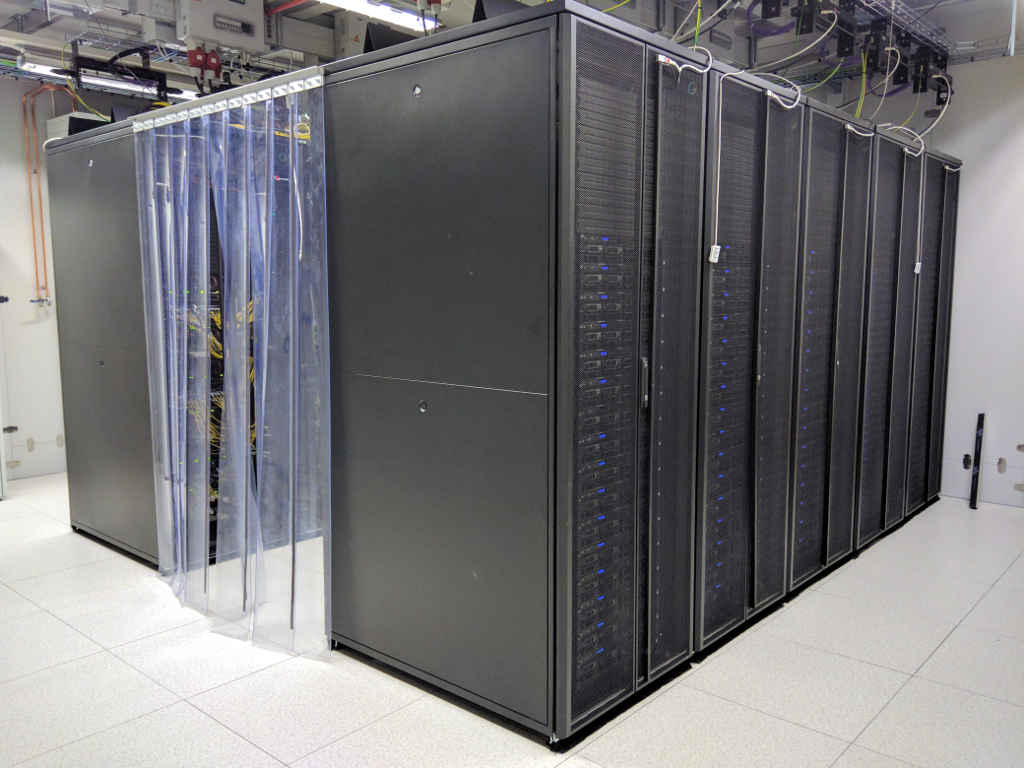
\includegraphics[width=1.0\linewidth]{pod2_interior.jpg}
\end{tiny}
\caption{Server racks in data center module POD 2 at RISE SICS North.}
\end{figure}
\end{column}%
\end{columns}
\end{frame}

%%%%%%%%%%%%%%%%%%%%%%%%%%%%%%%%%%%%%%%%%%%%%%%%%%%%%%%%%%%%%%%%%%%%%%%%
\begin{frame}{Data Centers}
\begin{columns}[T]% align columns
\begin{column}{.5\textwidth}
\begin{figure}[ht]
\begin{center}
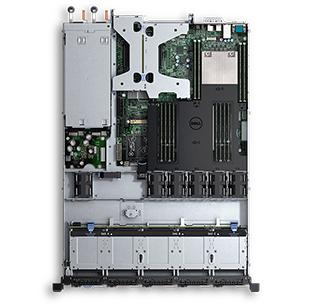
\includegraphics[width=1.2\linewidth]{dell_r430.jpg}
\end{center}
\caption{Dell R430 blade server with six internal fans.}
\end{figure}
\end{column}%
\hfill%
\begin{column}{.5\textwidth}
\begin{figure}[ht]
\begin{center}
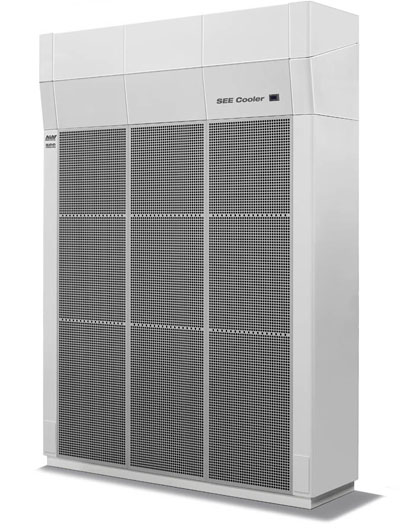
\includegraphics[width=0.95\linewidth]{crac.jpg}
\end{center}
\caption{Computer Room Air Conditioner, SEE Cooler HDZ-3.}
\end{figure}
\end{column}%
\end{columns}
\end{frame}

\section{The Lattice Boltzmann Method (LBM)}
%%%%%%%%%%%%%%%%%%%%%%%%%%%%%%%%%%%%%%%%%%%%%%%%%%%%%%%%%%%%%%%%%%%%%%%%
\begin{frame}{The Lattice Boltzmann Method (LBM)}
The LBM models the behavior of a group of particles as distribution functions in a uniform grid.
\begin{figure}[H]
\centering
\begin{scriptsize}
\def\svgwidth{\linewidth}
\input{Figures/scales.pdf_tex}
\end{scriptsize}
\caption{Techniques of simulations for different scales of fluid representations.}
\label{fig:scales}
\end{figure}
\end{frame}

%%%%%%%%%%%%%%%%%%%%%%%%%%%%%%%%%%%%%%%%%%%%%%%%%%%%%%%%%%%%%%%%%%%%%%%%
\begin{frame}{LBM: The Discrete Lattice Boltzmann Equation}
The evolution of the system is described by the Discrete Lattice Boltzmann Equation
\begin{equation} \label{eq:dbe}
f_i(\vec{x} + \vec{e_i}\Delta t, t + \Delta t) = f_i(\vec{x}, t) + \Gamma(f_i(\vec{x}, t)).
\end{equation}
Each distribution function $f_i$ is associated with a direction.

$\Gamma$ is called a collision operator and can be implemented in different ways. RAFSINE uses the Bhatnagar--Gross--Krook (BGK) method.

\end{frame}

%%%%%%%%%%%%%%%%%%%%%%%%%%%%%%%%%%%%%%%%%%%%%%%%%%%%%%%%%%%%%%%%%%%%%%%%
\begin{frame}{LBM: Streaming Step}
\begin{figure}[!htb]
\centering
\begin{minipage}[t]{.45\textwidth}
	\centering
	\begin{small}
	\def\svgwidth{0.9\linewidth}
	\input{Figures/d2q9_3.pdf_tex}
	\end{small}
	\caption{Lattice streaming step, representing advection in a fluid. All functions $f_i$ are copied to the neighboring $f_i^{temp}$ in parallel.}
	\label{fig:d2q9_3}
\end{minipage}\qquad%
\begin{minipage}[t]{.45\textwidth}
	\centering
	\begin{small}
	\def\svgwidth{0.9\linewidth}
	\input{Figures/d2q9_4.pdf_tex}
	\end{small}
	\caption{Also in the streaming step, the current site is filled with new distributions from the neighboring sites.}
	\label{fig:d2q9_4}
\end{minipage}
\end{figure}
\end{frame}

%%%%%%%%%%%%%%%%%%%%%%%%%%%%%%%%%%%%%%%%%%%%%%%%%%%%%%%%%%%%%%%%%%%%%%%%
\begin{frame}{LBM: Collision Step}
\begin{figure}[!htb]
\centering
\begin{minipage}[t]{.45\textwidth}
	\centering
	\begin{footnotesize}
	\def\svgwidth{0.9\linewidth}
	\input{Figures/d2q9_5.pdf_tex}
	\end{footnotesize}
	\caption{Collision step, representing diffusion in a fluid. Particles from adjacent sites collide locally in the current site (see BGK).}
	\label{fig:d2q9_5}
\end{minipage}\qquad%
\begin{minipage}[t]{.45\textwidth}
	\centering
	\begin{small}
	\def\svgwidth{0.9\linewidth}
	\input{Figures/d2q9_6.pdf_tex}
	\end{small}
	\caption{During the collide step the particle populations are redistributed. Both mass and momentum is conserved.}
	\label{fig:d2q9_6}
\end{minipage}
\end{figure}
\end{frame}

\section{RAFSINE}
%%%%%%%%%%%%%%%%%%%%%%%%%%%%%%%%%%%%%%%%%%%%%%%%%%%%%%%%%%%%%%%%%%%%%%%%
\begin{frame}{RAFSINE}

\begin{itemize}
\item Originally written by Nicolas Delbosc during his Ph.D study in the School of Mechanical Engineering at the
University of Leeds, England.
\item Implements LBM (BGK model) in C++ with streaming-, collision- and boundary-steps accelerated by Nvidia CUDA.
\item Simulates fluid behavior in real time or faster depending on domain size.
\item OpenGL visualization of system evolution.
\end{itemize}

\begin{figure}[ht]
\begin{center}
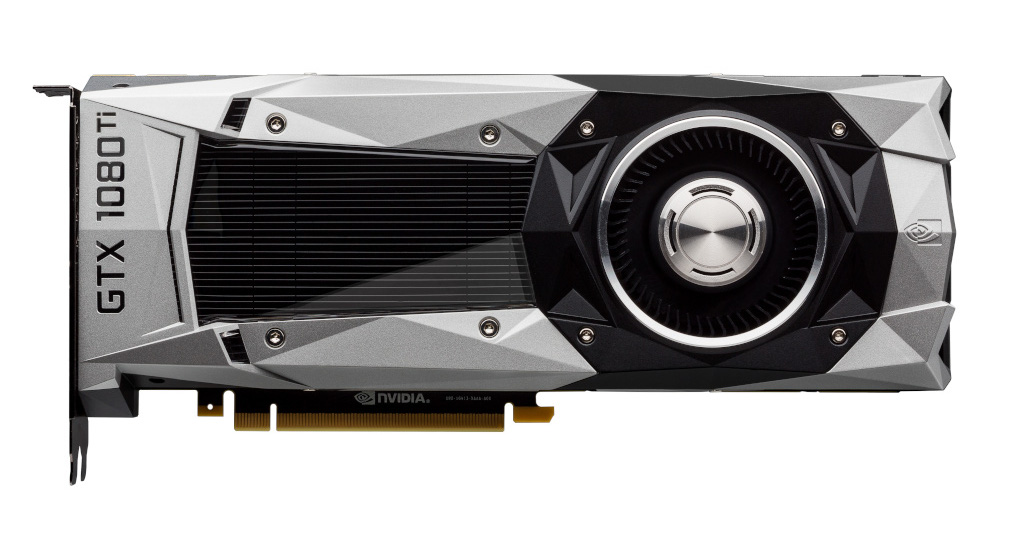
\includegraphics[width=0.5\linewidth]{1080ti.jpg}
\end{center}
\caption{Nvidia GTX 1080 Ti.}
\end{figure}

\end{frame}

%%%%%%%%%%%%%%%%%%%%%%%%%%%%%%%%%%%%%%%%%%%%%%%%%%%%%%%%%%%%%%%%%%%%%%%%
\begin{frame}{RAFSINE}

\begin{figure}[ht]
\begin{center}
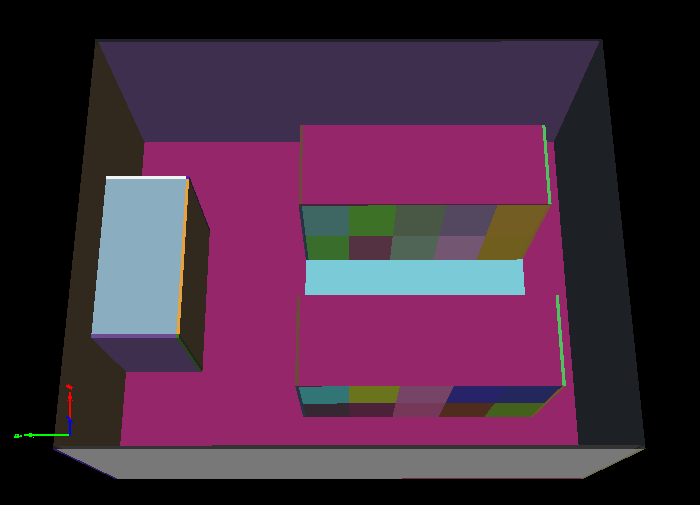
\includegraphics[width=0.9\linewidth]{voxels.png}
\end{center}
\caption{Geometry of an example data center.}
\label{fig:problem2}
\end{figure}

\end{frame}

%%%%%%%%%%%%%%%%%%%%%%%%%%%%%%%%%%%%%%%%%%%%%%%%%%%%%%%%%%%%%%%%%%%%%%%%
\begin{frame}{RAFSINE}

\begin{figure}[ht]
\begin{center}
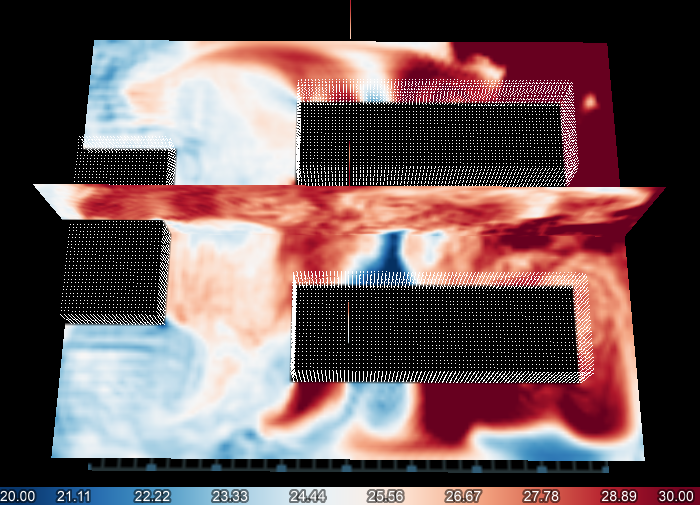
\includegraphics[width=0.9\linewidth]{temperature_halos.png}
\end{center}
\caption{Heat flow in an example data center.}
\label{fig:problem2}
\end{figure}

\end{frame}

%%%%%%%%%%%%%%%%%%%%%%%%%%%%%%%%%%%%%%%%%%%%%%%%%%%%%%%%%%%%%%%%%%%%%%%%
\begin{frame}{RAFSINE}

\begin{figure}[ht]
\begin{center}
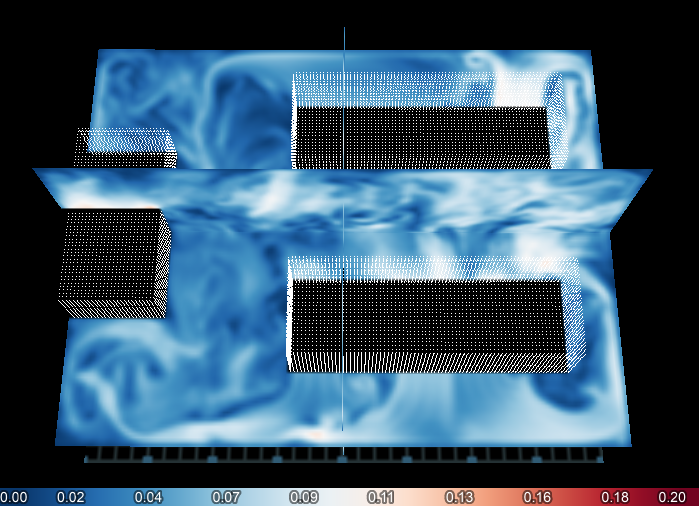
\includegraphics[width=0.9\linewidth]{velocity_halos.png}
\end{center}
\caption{Air velocity in an example data center.}
\label{fig:problem2}
\end{figure}

\end{frame}

\section{LBM on multiple GPUs}
%%%%%%%%%%%%%%%%%%%%%%%%%%%%%%%%%%%%%%%%%%%%%%%%%%%%%%%%%%%%%%%%%%%%%%%%
\begin{frame}{RAFSINE: Multiple GPUs}

\begin{figure}[ht]
\begin{center}
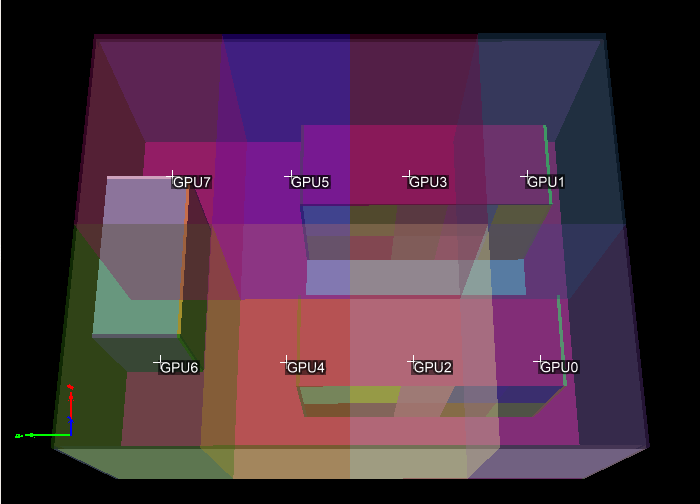
\includegraphics[width=0.9\linewidth]{voxels_gpus.png}
\end{center}
\caption{Domain decomposition of the data center.}
\label{fig:problem2}
\end{figure}

\end{frame}

%%%%%%%%%%%%%%%%%%%%%%%%%%%%%%%%%%%%%%%%%%%%%%%%%%%%%%%%%%%%%%%%%%%%%%%%
\begin{frame}{RAFSINE: Multiple GPUs}

\begin{figure}[ht]
\begin{center}
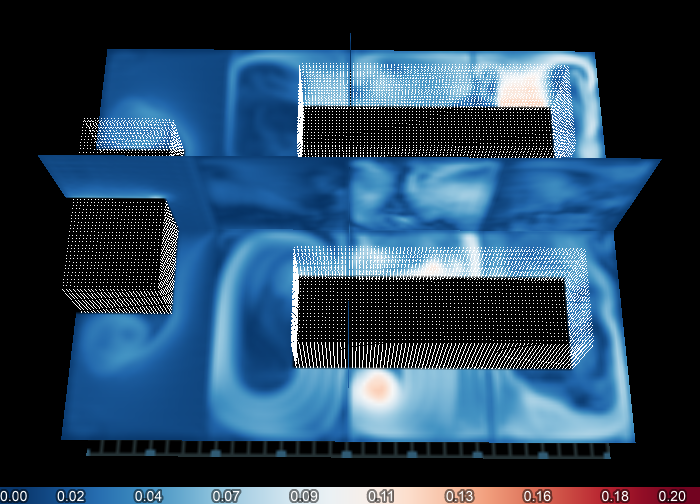
\includegraphics[width=0.9\linewidth]{velocity_nohalos.png}
\end{center}
\caption{Air velocity when decompositions are simulated separately.}
\label{fig:problem2}
\end{figure}

\end{frame}

%%%%%%%%%%%%%%%%%%%%%%%%%%%%%%%%%%%%%%%%%%%%%%%%%%%%%%%%%%%%%%%%%%%%%%%%
\begin{frame}{LBM: Halo Exchange}
Each GPU calculates the LBM evolution of a group of grid cells (lattice sites). After each evolution step, the state of the border sites (halos) are copied to buffers on neighbouring GPUs. These states are read in the next evolution.

\begin{figure}[!htb]
\centering
	\begin{tiny}
	\def\svgwidth{0.9\linewidth}
	\input{Figures/d3q19_halo_exchange.pdf_tex}
	\end{tiny}
	\caption{D3Q19 lattice site.}
	\label{fig:d2q9_1}
\end{figure}
Number of halos to copy depends on the type of lattice site.
\end{frame}


%%%%%%%%%%%%%%%%%%%%%%%%%%%%%%%%%%%%%%%%%%%%%%%%%%%%%%%%%%%%%%%%%%%%%%%%
\begin{frame}{LBM: Halo Exchange}
LBM discretizes the domain into a uniform grid of cells called lattice sites.
\begin{figure}[!htb]
\centering
\begin{minipage}[t]{.45\textwidth}
	\centering
	\begin{tiny}
	\def\svgwidth{0.9\linewidth}
	\input{Figures/d3q19.pdf_tex}
	\end{tiny}
	\caption{D3Q19 lattice site.}
	\label{fig:d2q9_1}
\end{minipage}\qquad%
\begin{minipage}[t]{.45\textwidth}
	\centering
	\begin{tiny}
	\def\svgwidth{0.9\linewidth}
	\input{Figures/d2q9_2.pdf_tex}
	\end{tiny}
	\caption{D2Q9 lattice site. Direction vectors $\vec{e}_i$ are lattice velocities, with their corresponding weight $w_i$.}
	\label{fig:d2q9_2}
\end{minipage}
\end{figure}
\end{frame}


%%%%%%%%%%%%%%%%%%%%%%%%%%%%%%%%%%%%%%%%%%%%%%%%%%%%%%%%%%%%%%%%%%%%%%%%
\begin{frame}{LBM: Halo Exchange}
\begin{itemize}
\item D3Q7 must copy \textbf{sides} to neighbours.
\item D3Q19 must copy \textbf{sides} and \textbf{edges}.
\item D3Q27 must copy \textbf{sides}, \textbf{edges} and \textbf{corners}.
\end{itemize}
\begin{figure}[!htb]
\centering
	\begin{tiny}
	\def\svgwidth{0.9\linewidth}
	\input{Figures/d3q19_halo_direction.pdf_tex}
	\end{tiny}
	\caption{Illustration of groups of lattice sites which must be copied to up to 26 neighbouring GPUs.}
	\label{fig:d2q9_1}
\end{figure}
\end{frame}


%%%%%%%%%%%%%%%%%%%%%%%%%%%%%%%%%%%%%%%%%%%%%%%%%%%%%%%%%%%%%%%%%%%%%%%%
\begin{frame}{RAFSINE: Multiple GPUs}
GPU to GPU communication is performed in a peer-to-peer fashion (NVIDIA GPUDirect). Data is transfered on the PCI-Express bus without passing through a CPU.
\begin{figure}[ht]
\begin{center}
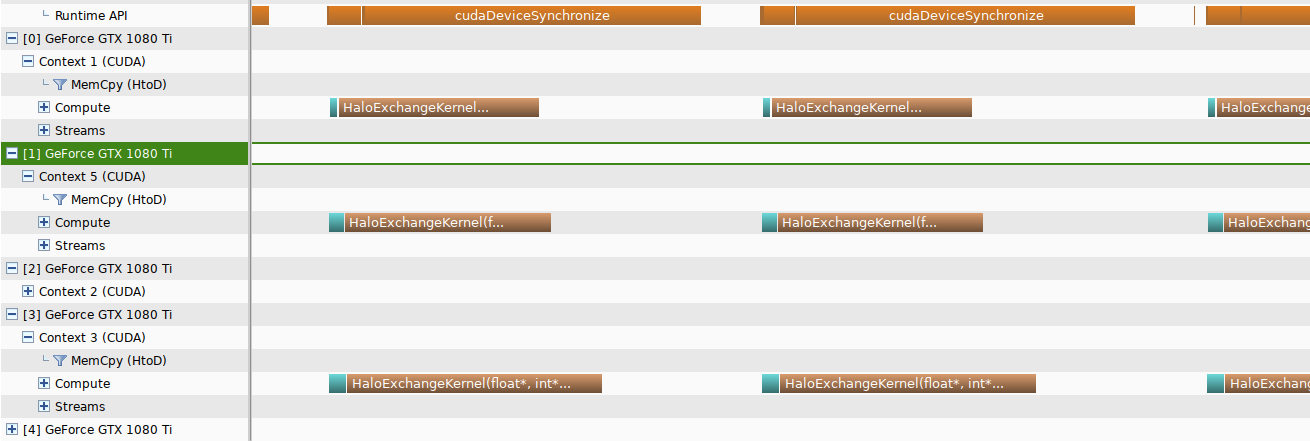
\includegraphics[width=1\linewidth]{nvvp.png}
\end{center}
\caption{NVIDIA Visual Profiler.}
\label{fig:problem2}
\end{figure}
This simple implementation works, but is limited by memory bandwidth. The amount of data can be reduced by only copying the distribution functions required by each neighbour.
\end{frame}

\section{Future work}
%%%%%%%%%%%%%%%%%%%%%%%%%%%%%%%%%%%%%%%%%%%%%%%%%%%%%%%%%%%%%%%%%%%%%%%%
\begin{frame}{Future work}
\begin{itemize}
\item Optimize halo exchange CUDA kernel and reduce amount of data copied.
\item Validate data center models of different sizes with measured data.
\item Develop Cascaded LBM and MRT into RAFSINE.
\item Develop a platform for training airflow control systems.
\end{itemize}
\end{frame}

%%%%%%%%%%%%%%%%%%%%%%%%%%%%%%%%%%%%%%%%%%%%%%%%%%%%%%%%%%%%%%%%%%%%%%%%
\begin{frame}{Thanks for listening!}

\end{frame}

\end{document}
